\documentclass[fleqn,a4paper,12pt]{article}

%used Packages
\usepackage{standalone}		% Zum Einlesen aus anderen .tex-Files
\usepackage{geometry}		% Zur Bearbeitung des Layouts (Ränder,...)
\usepackage[german]{babel}
\usepackage[utf8]{inputenc}
\usepackage{amsmath}		% Mathematische Symbole
\usepackage{amssymb}     	% Nochmehr mathematische Symbole
\usepackage{dsfont}      	% Schriftsatz fuer Zahlenmengensymbole
%\usepackage{verbatim}   	% erweiterte Verbatim-Umgebung
\usepackage{alltt}       	% Quasi-Verbatim-Umgebung
\usepackage{fancyhdr}    	% Eigene Kopfzeilen
\usepackage{graphicx}    	% Zum Einbinden von Grafiken
							% Einbinden einer eps-Grafik geht so: includegraphics{path}
\usepackage{wrapfig}
\usepackage{lscape}
\usepackage{rotating}
\usepackage{epstopdf}

% Skalierung der Grafiken
\setlength{\unitlength}{1cm}

\frenchspacing               % Kein Extrafreiraum nach Satzzeichen
\setlength{\parindent}{0pt}  % Neue Absaetze nicht einruecken
%\sloppy                     % Schlampige Absatzformatierung
\fussy                       % Penible Absatzformatierung
\linespread{1.5}             % Zeilenabstand


% Seitenraender
\geometry{left=30mm, right=40mm, bottom=30mm}
				% Doc-class, Packageimports, fancy stuff
%Seitenränder formatieren
\addtolength{\voffset}{-2cm}
\addtolength{\textheight}{0cm}
\addtolength{\hoffset}{0cm}
\addtolength{\textwidth}{2cm}
\addtolength{\headheight}{2cm} % fuer jeden Strichkode einen Zentimeter

% Font fuer Code 39
\font\xlix=wlc39 scaled 1200
\newcommand\barcode[1]{{\xlix@#1@}}

% Name, Matrikelnummer, Barcode
\newcommand\student[2]{
	\mbox{\scriptsize
		\begin{tabular}{@{}l@{}r@{}}
			\multicolumn{2}{@{}r@{}}{\barcode{#2}}\\
			#1&#2\\
		\end{tabular}}}

% Kopfzeile
\pagestyle{fancy}            % Eigene Kopfzeilen verwenden
\lhead{
	\small
	\textsc{Grundlagen der Signalverarbeitung \\
		WS 2017/2018 \\
		\"Ubung (\today)}
	\vfill}
\rhead{
	\begin{tabular}[b]{@{}rr@{}}
		\student{Philipp Badenhoop}{572693} &
		\student{Steven Lange}{568733} \\
		\student{Pascal Jochmann}{575056} &
		\student{Kevin Trogant}{572451}
\end{tabular}}			% Definition der Kopfzeile
%andere Definitionen
\providecommand{\R}{{\mathbb R}}
\providecommand{\N}{{\mathbb N}}
\providecommand{\Z}{{\mathbb Z}}
\providecommand{\Q}{{\mathbb Q}}
\providecommand{\C}{{\mathbb C}}
\providecommand{\F}{\mathcal{F}}
\providecommand{\less}{\setminus}
\providecommand{\inv}{{}^{-1}}
\providecommand{\Land}{\bigwedge}
\providecommand{\Lor}{\bigvee}			% Liste der zusätzlichen Commands und redefines

\begin{document}
	\section*{Aufgabe 24}
		\begin{itemize}
			\item[(a)] $T_A = 0.004s$\\
				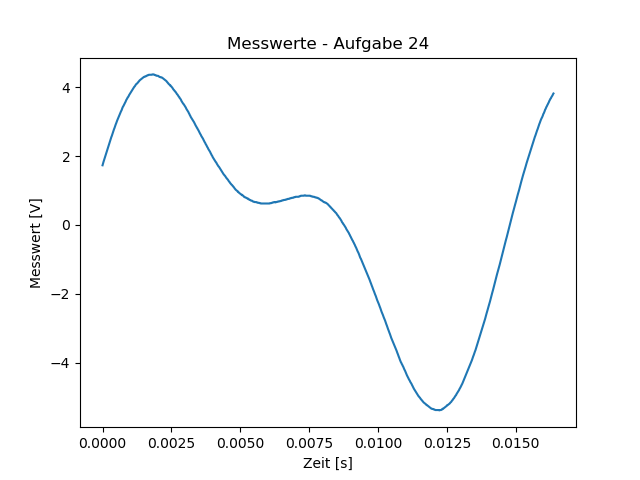
\includegraphics[scale = 0.7]{A24_messPlot.png}
			\item[(b)] $T_0 \approx 3.842s $\\
			$f_0 = \frac{1}{T_0} = 0.26Hz$\\
			$N = \left\lfloor \frac{3.842s}{0.004s} \right\rfloor = 960$\\
			$\omega_0 = \frac{2\pi}{N} \approx 0.0065\frac{rad}{s}$
			\item[(c)] Eine Periode mit $N$ Messwerte:\\
				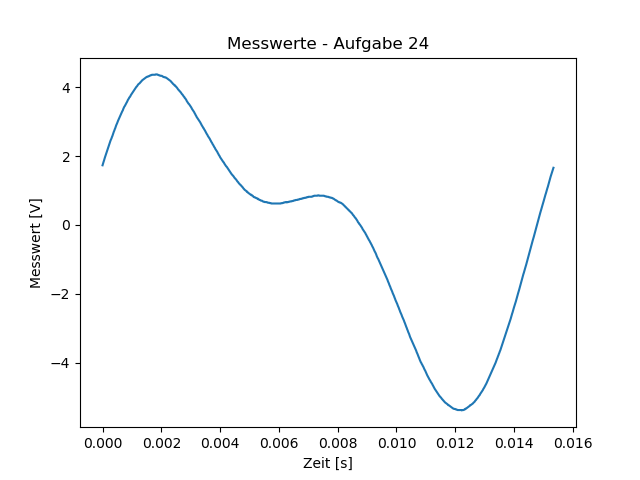
\includegraphics[scale = 0.7]{A24_messPlot_periode.png}
			\item[(d)] Für $k\in\{ 0, \pm 1, \pm 2, \dots \pm 15 \}$ gilt:
				$c_k = \frac{1}{960}\sum_{n=0}^{959} f_n\cdot e^{-j2\pi\frac{kn}{960}}$\\
			\begin{tabular}{c r r}
				k	&	$c_k$				&	$c_{-k}$\\
				0	&	-0.071				&	-0.071\\
				1	&	 0.226+1.809j		&	0.226-1.809j\\
				2	&	 0.667+0.772j		&	0.667-0.772j\\
				3	&	 0.000+0.003j		&	0.000-0.003j\\
				4	&	 0.000+0.001j		&	0.000-0.001j\\
				5	&	 0.000+0.001j		&	0.000-0.001j\\
				6	&	 0.001+0.001j		&	0.001-0.001j\\
				7	&	 0.001+0.000j		&	0.001+0.000j\\
				8	&	 0.001+0.000j		&	0.001+0.000j\\
				9	&	 0.001+0.001j		&	0.001-0.001j\\
				10	&	 0.000+0.000j		&	0.000+0.000j\\
				11	&	 0.000+0.001j		&	0.000-0.001j\\
				12	&	 0.000+0.001j		&	0.000-0.001j\\
				13	&	 0.000+0.001j		&	0.000-0.001j\\
				14	&	 0.000+0.000j		&	0.000+0.000j\\
				15	&	 0.000+0.001j		&	0.000-0.001j
			\end{tabular}
		\item[(d)] Das Linienspektrum sieht dann wie folgt aus:\\
			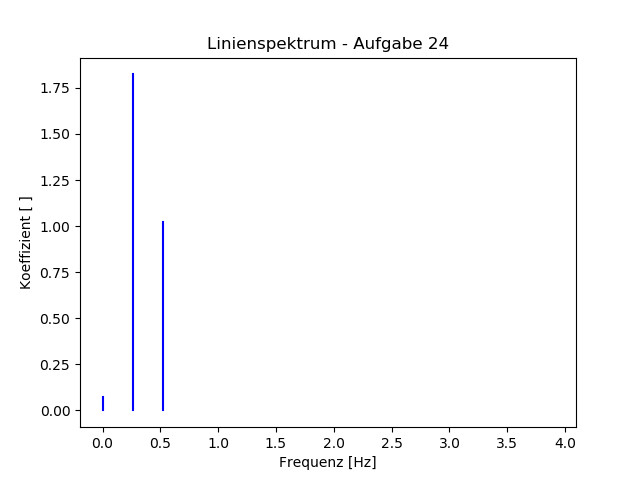
\includegraphics[scale = 0.7]{A24_Linienspektrum.png}
		\item[(e)] Das Signal ist zwar das Beispiel-Signal aus der Vorlesung und der Übung, aber welches dies genau ist, ist uns unbekannt.	
	\end{itemize}
\newpage
	\section*{Aufgabe 25}
		$d = 0.2$\\
		$T_0 = 1$\\
		$\omega_0 = 2\pi$\\
		Tastgrad $= \frac{\text{Impulsdauer}}{T_0} = \frac{2d}{T_0} = 0.4$\\
		Gleichanteil $= \int_{a}^{a+T_0} f(t) dt = 0.4$\\
		Entwicklungsintervall $=$ \glqq sicheres Orthogonalitätsintervall\grqq\ $= \left[-\frac{T_0}{2},\frac{T_0}{2}\right]$\\
        %
        Die approximierte Funktion ergibt sich durch:
        \begin{align*}
            f_{ap}(t) &= \frac{a_0}{2} + \sum_{k=1}^\infty \left(a_k \cdot \cos(2\pi \omega_0 t) + b_k \cdot \sin(2\pi \omega_0 t)\right) \\
            \text{mit:} \\
            a_k &= 2 \int_{0}^{1} f(t) \cos(2\pi k t) \, \text{d}t = 2 \int_{0}^{0.2} \cos(2\pi k t) \, \text{d}t = 2 \left[ \frac{\sin(2\pi k t)}{2\pi k} + C_0 \right]_0^{0.2} \\
            b_k &= 2 \int_{0}^{1} f(t) \sin(2\pi k t) \, \text{d}t = 2 \int_{0}^{0.2} \sin(2\pi k t) \, \text{d}t = 2 \left[ \frac{-\cos(2\pi k t)}{2\pi k} + C_1 \right]_0^{0.2}
        \end{align*}
        % 
        \begin{figure}
            \includegraphics[width=\textwidth]{A25_plot.png}
            \caption{Darstellung für verschiedene $k$ im Intervall $t = 0 \dots 0.4$}
        \end{figure}
        %
        \begin{figure}
            \includegraphics[width=\textwidth]{A25_plot2.png}
            \caption{Linienspektrum für verschiedene Tastgrade}
        \end{figure}
\newpage
	\section*{Übungsaufgabe 26:}
	Berechnete Koeffizienten mit dem Verfahren aus 1921:\newline
	\begin{center}
		\begin{tabular}{|c|c|c|}
			\hline 
			$k$ & $a_k$ & $b_k$ \\
			\hline
			0   &  128.55    & 0 \\
			1   &  77.9    & 62.6 \\
			2   &  1.3    & 1.9 \\
			3   &  -31.5    & -11.1 \\
			4   &  -1.9    & -1.4 \\
			5   &  0.5    & 1.4 \\
			6   &  0.3    & 11.6 \\
			7   &  -1    & 0 \\
			8   &  -0.5    & -0.5 \\
			9   &  0.9    & 1.2 \\
			\hline
		\end{tabular}
	\end{center}
	Berechnete Koeffizienten mit Matlab:
	\begin{center}
		\begin{tabular}{|c|c|c|}
			\hline 
			$k$ & $a_k$ & $b_k$ \\
			\hline
			0   &  257.1    & 0 \\
			1   &  78    & 62.6 \\
			2   &  1    & 1.76 \\
			3   &  -32    & -10.8 \\
			4   &  -1    & -1.35 \\
			5   &  0.5    & 1.4 \\
			6   &  0.28    & 1.15 \\
			7   &  -0.64    & -1.6 \\
			8   &  0.45    & -0.57 \\
			9   &  0.72    & 1.17 \\
			\hline
		\end{tabular}
	\end{center}
	An dieser Stelle sei gesagt, dass wir mit Matlab die Koeffizienten wiederum durch die Fouriersynthese überprüft haben.
	Im Vergleich sind die Werte bis mit 0 < k < 6 sehr ähnlich, wobei der Rest deutliche Abweichungen zeigt.l
	
\newpage\end{document}